\section{Supervised Binary Classification Results}\label{Chapter-3-Supervised}
\noindent We evaluate the supervised binary text classification performance (Human vs. AI) on our test set. We compare a lightweight lexical baseline (FastText) against our fine-tuned DistilBERT transformer classifier:

\begin{table}[h]
\centering
\begin{tabular}{lccccc}
\toprule
\textbf{Model} & \textbf{Accuracy} & \textbf{AUC} & \textbf{Precision} & \textbf{Recall} & \textbf{F1-Score} \\
\midrule
FastText Baseline & 64.6\% & 0.711 & 67.1\% & 57.3\% & 0.618 \\
DistilBERT Classifier & \textbf{78.4\%} & \textbf{0.925} & \textbf{91.9\%} & \textbf{62.2\%} & \textbf{0.742} \\
\bottomrule
\end{tabular}
\caption{Supervised binary classifier performance on test set.}
\label{tab:supervised_results}
\end{table}

\noindent The DistilBERT classifier significantly outperforms the FastText baseline. It achieves an AUC of $0.925$ and maintains a high precision of $91.9\%$, prioritizing the prevention of "false accusations" (labeling human text as AI).

\section{Baseline Detection Paradigms}\label{Chapter-3-Paradigms}
We implement four detection approaches to compare paradigms:
\begin{enumerate}
    \item \textbf{FastText (Lexical):} Matches character and word n-gram frequencies. Fast but lacks context awareness.
    \item \textbf{GLTR (Predictability):} Measures word probability ranks under GPT-2. Exploits the fact that LLMs choose highly predictable words (top ranks), whereas humans write with higher entropy.
    \item \textbf{DetectGPT-lite (Zero-Shot Curvature):} Perturbs the text using DistilRoBERTa-base and measures likelihood differences under GPT-2. Zero-shot but computationally expensive.
    \item \textbf{DistilBERT (Contextual):} Processes text bidirectionally to capture subtle stylistic footprints.

\end{enumerate}

\section{Proposed Open-Set Rejection Layer}\label{Chapter-3-Novelty}
\noindent To identify and reject text generated by unseen models, we build a Stage-2 open-set rejection layer based on known class distributions.

\subsection{Mathematical Formulation}
For each known class $c \in \{0, 1\}$ (representing known generators GPT and LLaMA), we extract training embeddings $\mathbf{x} \in \mathbb{R}^{768}$ and compute the class centroid:
$$\mu_c = \frac{1}{N_c} \sum_{i=1}^{N_c} \mathbf{x}_i^{(c)}$$
We compute the regularized class covariance matrix:
$$\Sigma_c = \text{Cov}(X^{(c)}) + 10^{-4} \cdot I_{768}$$
The out-of-distribution (OOD) score of a test embedding $\mathbf{z}$ is defined as the minimum Mahalanobis distance to known class distributions:
$$D(\mathbf{z}) = \min_{c \in \{0, 1\}} \sqrt{(\mathbf{z} - \mu_c)^T \Sigma_c^{-1} (\mathbf{z} - \mu_c)}$$
The OOD threshold $\tau$ is chosen as the **95th percentile** of the known validation set's minimum Mahalanobis distances.

\begin{figure}[H]
\centering
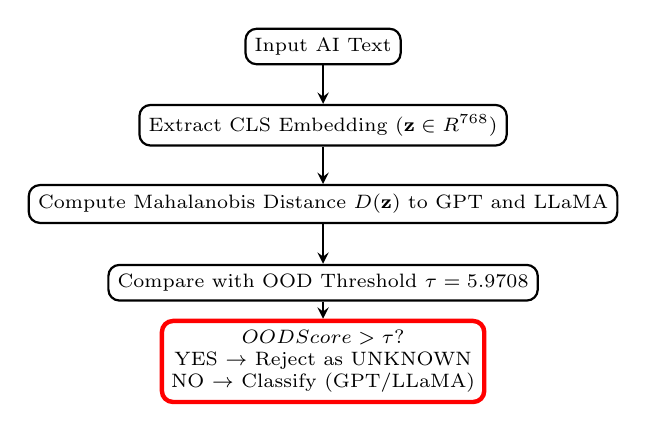
\begin{tikzpicture}[node distance=1.0cm, every node/.style={fill=white, draw=black, rounded corners, thick, align=center, font=\scriptsize}, arrow/.style={thick, ->, >=stealth}]
\node (input) {Input AI Text};
\node (cls) [below of=input] {Extract CLS Embedding ($\mathbf{z} \in \mathbb{R}^{768}$)};
\node (dist) [below of=cls] {Compute Mahalanobis Distance $D(\mathbf{z})$ to GPT and LLaMA};
\node (thresh) [below of=dist] {Compare with OOD Threshold $\tau = 5.9708$};
\node (decision) [below of=thresh, draw=red, ultra thick] {$\text{OOD Score} > \tau$? \\ YES $\to$ Reject as UNKNOWN \\ NO $\to$ Classify (GPT/LLaMA)};

\draw [arrow] (input) -- (cls);
\draw [arrow] (cls) -- (dist);
\draw [arrow] (dist) -- (thresh);
\draw [arrow] (thresh) -- (decision);
\end{tikzpicture}
\caption{Open-set generator rejection pipeline flow.}
\label{fig:pipeline_flow}
\end{figure}

\section{Baseline Open-Set Rejection Results}\label{Chapter-3-Baseline}
In our baseline configuration (unseen: OPT, known: GPT + LLaMA, representation: CLS, distance: Mahalanobis):
\begin{itemize}
    \item \textbf{Selected Threshold ($\tau$):} $63.5972$
    \item \textbf{OPT Unknown Rejection Rate:} $7.59\%$ (608 / 8,012 OPT samples flagged)
    \item \textbf{Known Class False Rejection:} $3.90\%$ (39 / 1,000 known test samples incorrectly flagged)
    \item \textbf{OOD Score AUROC:} $0.6298$
\end{itemize}
The baseline OOD AUROC ($0.6298$) represents modest separation. While it maintains a low false rejection rate, only a small fraction of the unseen OPT family is successfully rejected.

\section{Experiment 1: Representation Pooling Study}\label{Chapter-3-Exp1}
We evaluate the representation extraction method, comparing CLS token pooling against attention-mask-aware mean pooling:
\begin{table}[h]
\centering
\begin{tabular}{lccc}
\toprule
\textbf{Metric} & \textbf{Baseline (CLS Pooling)} & \textbf{Experiment 1 (Mean Pooling)} & \textbf{Delta} \\
\midrule
\textbf{Unseen OPT Rejection} & \textbf{7.59\%} & \textbf{1.61\%} & -5.98\% \\
\textbf{Known False Rejection} & \textbf{3.90\%} & \textbf{4.40\%} & +0.50\% \\
\textbf{Open-Set OOD AUROC} & \textbf{0.6298} & \textbf{0.5251} & -0.1047 \\
\textbf{OOD Threshold} & 63.5972 & 5.8443 & -57.7529 \\
\bottomrule
\end{tabular}
\caption{Experiment 1 representation pooling results.}
\label{tab:exp1_results}
\end{table}

\noindent Mean pooling drops performance to near-random ($0.5251$ AUROC). Since classification fine-tuning concentrates style features into the \texttt{[CLS]} token, averaging across all tokens averages in semantic domain signatures, washing out generator styles.

\section{Experiment 2: Distance Metric Study}\label{Chapter-3-Exp2}
We compare Mahalanobis distance against Cosine distance:
\begin{table}[h]
\centering
\begin{tabular}{lccc}
\toprule
\textbf{Metric} & \textbf{Baseline (Mahalanobis)} & \textbf{Experiment 2 (Cosine)} & \textbf{Delta} \\
\midrule
\textbf{Unseen OPT Rejection} & \textbf{7.59\%} & \textbf{0.85\%} & -6.74\% \\
\textbf{Known False Rejection} & \textbf{3.90\%} & \textbf{3.70\%} & -0.20\% \\
\textbf{Open-Set OOD AUROC} & \textbf{0.6298} & \textbf{0.4898} & -0.1400 \\
\textbf{OOD Threshold} & 63.5972 & 0.0158 & -63.5814 \\
\bottomrule
\end{tabular}
\caption{Experiment 2 distance metric results.}
\label{tab:exp2_results}
\end{table}

\noindent Cosine distance collapses completely (AUROC = $0.4898$, below random). Fine-tuning collapses embeddings into a collinear cone. Without covariance scaling to expand style variations, angular distance cannot separate the distributions.

\section{Experiment 3: Generalization Study}\label{Chapter-3-Exp3}
We evaluate three leave-one-generator-out configurations under strict no-leakage partitions:
\begin{table}[h]
\footnotesize
\centering
\begin{tabular}{lccc}
\toprule
\textbf{Metric} & \textbf{3A: OPT unseen} & \textbf{3B: LLaMA unseen} & \textbf{3C: GPT unseen} \\
\midrule
\textbf{Known Generators} & GPT + LLaMA & GPT + OPT & LLaMA + OPT \\
\textbf{Unseen Generator} & OPT & LLaMA & GPT \\
\textbf{Threshold} & \textbf{5.9708} & \textbf{57.8356} & \textbf{72.8708} \\
\textbf{Unknown Rejection} & \textbf{1.41\%} & \textbf{5.12\%} & \textbf{27.85\%} \\
\textbf{Known False Rejection} & \textbf{4.10\%} & \textbf{6.40\%} & \textbf{5.80\%} \\
\textbf{OOD AUROC} & \textbf{0.5263} & \textbf{0.4919} & \textbf{0.7587} \\
\bottomrule
\end{tabular}
\caption{Experiment 3 cross-generator generalization results.}
\label{tab:exp3_results}
\end{table}

\noindent GPT is highly separable ($0.7587$ AUROC, $27.85\%$ rejection) because its proprietary alignment differs substantially from open models. LLaMA unseen collapses ($0.4919$ AUROC) due to structural overlap with the OPT family in pre-training.

\section{Domain-Wise Performance Analysis}\label{Chapter-3-Domains}
We break down the OOD AUROC performance across writing domains:
\begin{table}[h]
\centering
\begin{tabular}{lccc}
\toprule
\textbf{Unseen Generator} & \textbf{XSum AUROC} & \textbf{ELI5 AUROC} & \textbf{WritingPrompts AUROC} \\
\midrule
OPT (3A) & 0.5307 & 0.5340 & 0.4698 \\
LLaMA (3B) & 0.4555 & 0.3963 & 0.5609 \\
GPT (3C) & \textbf{0.6665} & \textbf{0.8006} & \textbf{0.7836} \\
\bottomrule
\end{tabular}
\caption{Domain-wise OOD score AUROC across leave-one-out configurations.}
\label{tab:domain_auroc}
\end{table}

\noindent Open-set performance varies heavily across writing styles, with creative writing (WritingPrompts) and forum answers (ELI5) showing much stronger OOD separation for GPT than news articles (XSum).
